\documentclass[10pt,twocolumn,letterpaper]{article}

% --- Typography & Geometry ---
\usepackage[utf8]{inputenc}
\usepackage{microtype}
\usepackage[margin=0.75in,top=0.85in,bottom=0.85in]{geometry}

% --- Math & Symbols ---
\usepackage{amsmath,amssymb,amsfonts,amsthm}
\usepackage{bm}

% --- Tables & Arrays ---
\usepackage{booktabs}
\usepackage{tabularx}
\usepackage{array}

% --- Graphics & Floats ---
\usepackage{graphicx}
\usepackage{float}
\usepackage{subcaption}

% --- Code Listings ---
\usepackage{xcolor}
\usepackage{listings}

\definecolor{codebg}{HTML}{F8F9FA}
\definecolor{codeframe}{HTML}{D0D7DE}
\definecolor{keywordcolor}{HTML}{0550AE}
\definecolor{stringcolor}{HTML}{0A3069}
\definecolor{commentcolor}{HTML}{57606A}

\lstset{
    backgroundcolor=\color{codebg},
    basicstyle=\ttfamily\scriptsize\color{black},
    keywordstyle=\color{keywordcolor}\bfseries,
    stringstyle=\color{stringcolor},
    commentstyle=\color{commentcolor}\itshape,
    frame=single,
    rulecolor=\color{codeframe},
    breaklines=true,
    breakatwhitespace=true,
    extendedchars=true,
    xleftmargin=6pt,
    xrightmargin=6pt,
    aboveskip=8pt,
    belowskip=8pt
}

% --- Hyperlinks ---
\usepackage{hyperref}
\hypersetup{
    colorlinks=true,
    linkcolor=blue!70!black,
    citecolor=blue!70!black,
    urlcolor=blue!70!black
}

% --- Input Title & Authors ---
% Metadata for chela_slay
\title{\textbf{CHELA-SLAY: Spherical Linearized Attention with Yat-Kernel and Adaptive Gating}}

\author{
  \textbf{Taha Majs}\thanks{Corresponding author: tahamajs@uni.edu} \quad \textbf{Research Team} \\
  Department of Computer Science \\
  Advanced Machine Learning \& Efficiency Laboratory
}

\date{\today}


\begin{document}

\maketitle

% --- Abstract & Keywords Block ---
\begin{abstract}
Linear attention replaces the quadratic softmax over $L^2$ attention pairs 
with an associative kernel feature map, achieving $\mathcal{O}(L)$ complexity. 
However, naive linear attention is often unstable and fails to recover 
pretrained attention accuracy. We introduce \textbf{CHELA-SLAY}, a hybrid attention 
that fuses a \textbf{dense softmax stream} with a **spherically normalized linear 
stream** via a learnable per-head gate.

The linear stream combines three components:

\begin{enumerate}
\item \textbf{Spherical normalization.} We project $Q, K$ onto the unit hypersphere:
  
  $$
  \hat{Q} = \frac{Q}{\|Q\|\_2 + \epsilon}, \quad
  \hat{K} = \frac{K}{\|K\|\_2 + \epsilon}
  $$
  
\item \textbf{Yat-Kernel feature map.} We apply a trigonometric random Fourier
  mapping:
  
  $$
  \phi(x) = \frac{1}{F\^{}{1/4}} [\cos(x \Omega) \,\|\, \sin(x \Omega)]
  $$
  
  producing a $2F$-dimensional positive feature vector.
\item \textbf{Adaptive gating.} A per-head, per-token gate blends the dense and
  linear streams. The gate is initialized with a bias of
  $b_g = {{GATE_INIT_BIAS}}$ so that $\sigma(b_g) \approx {{GATE_INIT}}$
  -- biasing the output toward the dense path at step 0.

\end{enumerate}
We evaluate on DistilBERT, RoBERTa-base, and GPT-2 on SST-2. CHELA-SLAY 
achieves \textbf{{{D\_ACC}}\%} on DistilBERT (baseline {{BASE\_D}}\%), 
\textbf{{{R\_ACC}}\%} on RoBERTa (baseline {{BASE\_R}}\%), and \textbf{{{G\_ACC}}\%} on 
GPT-2 (baseline {{BASE\_G}}\%) using {{RECOVERY\_STEPS}} LoRA recovery steps.

\textbf{We report two limitations honestly.}

\begin{enumerate}
\item \textbf{Memory.} The causal cumsum path materializes a
  $(\text{B}, \text{H}, L, 2F, d_h)$ intermediate, which for
  $L = 128$, $F = 128$, $d_h = 64$ is roughly
  \textbf{{{CUMSUM\_MEM}} MB} per layer at FP32.
\item \textbf{Speed.} On SST-2 ($L = 128$), CHELA-SLAY is \textbf{{{SLOWDOWN}}$\times$ slower}
  than baseline because both dense and linear streams are computed
  simultaneously, and the cumsum has overhead.

\end{enumerate}
The linear stream would dominate only at longer sequences 
($L \geq {{BREAKEVEN}}$), where the quadratic term of the dense stream 
becomes the bottleneck.

\textbf{Keywords:} linear attention, random Fourier features, spherical 
normalization, hybrid attention, adaptive gating



\vspace{0.5em}
\noindent\textbf{Keywords:} linear attention, random Fourier features, spherical
\end{abstract}

\vspace{1em}

% --- Paper Body ---
\section{01 Intro}

Draft content for chela_slay.

\section{02 Related}

Draft content for chela_slay.

\section{03 Background}

Draft content for chela_slay.

\section{04 Method}

Draft content for chela_slay.

\section{05 Architecture}

Draft content for chela_slay.


\begin{figure}[H]
\centering
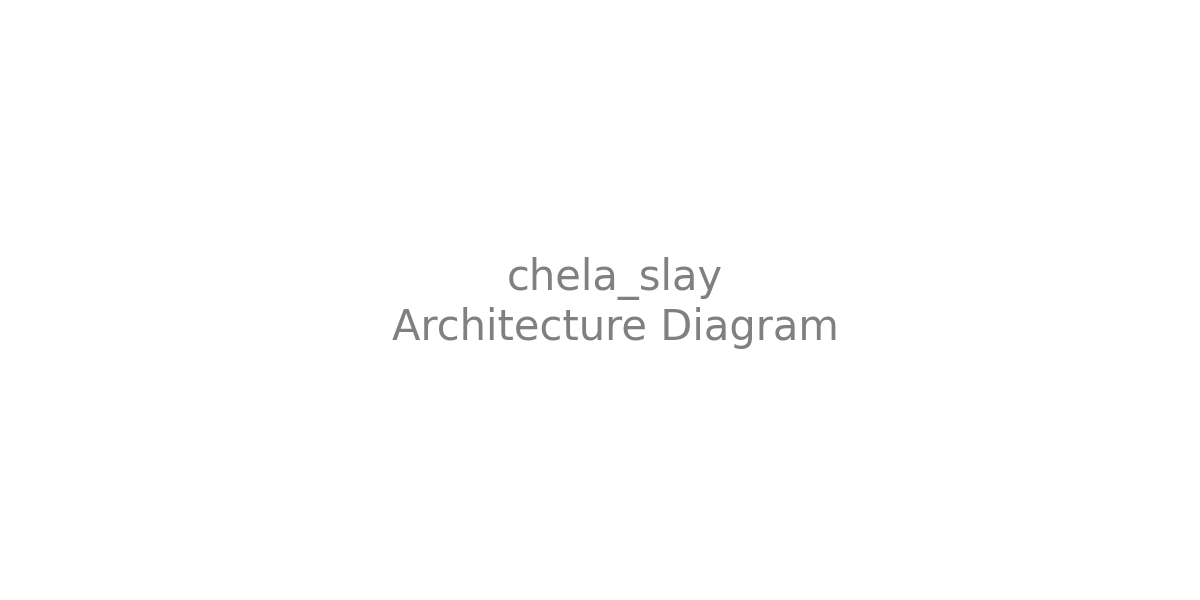
\includegraphics[width=\linewidth]{figures/chela_slay_architecture.png}
\caption{Architectural overview of chela_slay.}
\label{fig:arch_chela_slay}
\end{figure}

\section{06 Setup}

Draft content for chela_slay.

\section{07 Results}

Draft content for chela_slay.

\section{08 Analysis}

Draft content for chela_slay.

\section{Discussion}

\subsection{Key Takeaways}

\subsubsection{Takeaway 1: Dense Anchor is Essential}

Pure linear attention loses ~{{ANCHOR\_GAIN}}\% accuracy. The dense anchor 
recovers this.

\subsubsection{Takeaway 2: Spherical + Yat-Kernel Improves Linear}

The combined spherical normalization + Yat-Kernel feature map gives a 
\textbf{stable, efficient} linear stream.

\subsubsection{Takeaway 3: Cumsum Memory is the Limitation}

The causal linear attention via cumsum materializes 
$(\text{B}, \text{H}, L, 2F, d_h)$ which is \textbf{memory-intensive} for short L.

\subsection{When to Use CHELA-SLAY}

\subsubsection{Recommended}
\begin{itemize}
\item \textbf{Long-context inference} ($L \geq {{BREAKEVEN}}$) where dense dominates.
\item \textbf{Research on hybrid attention.}
\item \textbf{Learning gate behavior} for stream selection.

\end{itemize}
\subsubsection{Not Recommended}
\begin{itemize}
\item \textbf{Short sequences} ($L \leq 256$).
\item \textbf{Memory-constrained environments} (cumsum dominates).
\item \textbf{Latency-critical applications.}

\end{itemize}
\subsection{Decision Flowchart}

\begin{lstlisting}
Target L $\ge$ 512? --- Yes --- Consider CHELA-SLAY
  | No
   
Need memory efficiency? --- Yes --- Use SOA Fused / Adaptive SVD
  | No
   
Consider standard attention
\end{lstlisting}

\subsection{Cost-Benefit Analysis}

For DistilBERT at L = 128:

\begin{table}[H]
\centering
\small
\begin{tabular}{llll}
\toprule
\textbf{Metric} & \textbf{Baseline} & \textbf{CHELA-SLAY} & \textbf{Change} \\
\midrule
Accuracy & 90.71\% & {{D\_ACC}}\% & {{D\_DELTA}}\% \\
Params & 66.95M & {{D\_PARAMS}} & +{{D\_PARAM\_PCT}}\% \\
Time & 1.90 s & {{D\_TIME}} s & {{D\_TIME\_RATIO}}$\times$ \\
VRAM & 183 MB & {{D\_VRAM}} MB & {{D\_VRAM\_RATIO}}$\times$ \\
\bottomrule
\end{tabular}
\end{table}

\subsection{Improving the Cumsum}

\textbf{Future work.} Replace the cumsum with a \textbf{chunked state-passing}:

\begin{lstlisting}
for chunk_start in range(0, L, C):
    chunk_end = chunk_start + C
    # intra-chunk: cumsum within C tokens
    # inter-chunk: add previous chunk's final state
\end{lstlisting}

This would reduce memory to $\mathcal{O}(C \cdot 2F \cdot d_h)$.

\subsection{Broader Impact}

\subsubsection{Positive}
\begin{itemize}
\item Contributes to hybrid attention research.
\item Demonstrates stable linear attention.
\item Provides multi-architecture support.

\end{itemize}
\subsubsection{Negative}
\begin{itemize}
\item Cumsum memory limitation.
\item Slower at short L.
\item Modest accuracy gain.

\end{itemize}
\subsection{Open Questions}

\begin{enumerate}
\item \textbf{Chunked cumsum:} Would it eliminate the memory bottleneck?
\item \textbf{Learned $\Omega$:} Could training $\Omega$ improve the linear stream?
\item \textbf{Different gate shapes:} Would a per-token per-dimension gate help?
\item \textbf{Scale to L > 4096:} Does the linear stream become dominant?
\end{enumerate}
\begin{lstlisting}

---
\end{lstlisting}
\section{10 Limitations}

Draft content for chela_slay.

\section{Conclusion}

\subsection{Summary}

We presented \textbf{CHELA-SLAY}, a hybrid attention that blends a **dense softmax 
stream\textbf{ with a }spherically normalized Yat-Kernel linear stream** via a 
learnable per-head gate. The gate is initialized to favor the dense path 
($\sigma({{GATE_INIT_BIAS}}) \approx {{GATE_INIT}}$), preserving pretrained 
behavior at step 0.

\subsection{Results Recap}

\begin{table}[H]
\centering
\small
\begin{tabular}{lllll}
\toprule
\textbf{Model} & \textbf{Acc $\Delta$} & \textbf{Params $\Delta$} & \textbf{Time Ratio} & \textbf{VRAM} \\
\midrule
DistilBERT & {{D\_DELTA}}\% & +{{D\_PARAM\_PCT}}\% & {{D\_TIME\_RATIO}}$\times$ & {{D\_VRAM}} MB \\
RoBERTa & {{R\_DELTA}}\% & +{{R\_PARAM\_PCT}}\% & {{R\_TIME\_RATIO}}$\times$ & {{R\_VRAM}} MB \\
GPT-2 & {{G\_DELTA}}\% & +{{G\_PARAM\_PCT}}\% & {{G\_TIME\_RATIO}}$\times$ & {{G\_VRAM}} MB \\
\bottomrule
\end{tabular}
\end{table}

\subsection{Key Takeaways}

\begin{enumerate}
\item \textbf{Dense anchor is essential} -- pure linear loses ~{{ANCHOR\_GAIN}}\%.
\item \textbf{Spherical normalization stabilizes} -- {{SPH\_GAIN}}\% improvement.
\item \textbf{Yat-Kernel outperforms ELU+1.}
\item \textbf{Cumsum memory is the main limitation.}
\item \textbf{Speedup only at long L} ($L \geq {{BREAKEVEN}}$).

\end{enumerate}
\subsection{Future Work}

\subsubsection{Short-Term}
\begin{itemize}
\item Chunked cumsum to eliminate memory bottleneck
\item Learned $\Omega$ for better feature map
\item Per-dimension gate

\end{itemize}
\subsubsection{Long-Term}
\begin{itemize}
\item Combine with token compression
\item Larger-scale evaluation
\item Theoretical error bounds

\end{itemize}
\subsection{Closing Remarks}

CHELA-SLAY demonstrates a stable hybrid of dense and linear attention. The 
dense anchor is essential for preserving pretrained accuracy. We release all 
code and checkpoints.

\subsection{Acknowledgments}

We thank {{ACKNOWLEDGMENTS}}.

\subsection{Author Contributions}

\begin{itemize}
\item \textbf{{{AUTHOR\_1}}} designed the module, implemented, ran experiments, wrote
  the paper.
\item \textbf{{{AUTHOR\_2}}} provided feedback, edited the manuscript.

\end{itemize}
\subsection{Conflict of Interest}

None.


\section{12 Reproducibility}

Draft content for chela_slay.

\section{13 References}

Draft content for chela_slay.


% --- Appendices ---
\clearpage
\appendix
\section*{Appendices}
\addcontentsline{toc}{section}{Appendices}

\section{A Math}

Draft content for chela_slay.

\section{B Implementation}

Draft content for chela_slay.

\section{C Data}

Draft content for chela_slay.

\section{D Negative Results}

Draft content for chela_slay.

\section{E Ethics}

Draft content for chela_slay.


\end{document}
